\documentclass[12pt]{article}
\usepackage{enumitem}
\usepackage{setspace}
\usepackage{graphicx}
\usepackage{subfig}
\usepackage{booktabs}
\usepackage{amsmath, amsthm}
\RequirePackage[colorlinks]{hyperref}
\usepackage[lined,boxed,linesnumbered,commentsnumbered]{algorithm2e}
\usepackage{xcolor}
\usepackage{listings}
\usepackage{float}
\lstset{basicstyle=\ttfamily,
  showstringspaces=false,
  commentstyle=\color{red},
  keywordstyle=\color{blue}
}

% Margins
\topmargin=-0.45in
\evensidemargin=0in
\oddsidemargin=0in
\textwidth=6.5in
\textheight=9.0in
\headsep=0.25in

\linespread{1.1}

% Commands
\newenvironment{solution}
  {\begin{proof}[Solution]}
  {\end{proof}}

\newcommand{\snehaedit}[1]{\textcolor{green}{\emph{[Sneha: #1]}}}
\newcommand{\hsedit}[1]{\textcolor{magenta}{\emph{[Hang: #1]}}}
\newcommand{\meeraedit}[1]{\textcolor{red}{\emph{[Meera: #1]}}}
\newcommand{\prpedit}[1]{\textcolor{blue}{\emph{[Prp: #1]}}}


\title{CSE6250: Big Data Analytics in Healthcare \\ Homework 2 Answers}
\author{Richard Albright}
\date{Deadline: Feb 14, 2021, 11:55 PM AoE}

\begin{document}

\maketitle
\begin{itemize}
\item Discussion is encouraged, but each student must write his/her own answers and explicitly mention any collaborators.
\item Each student is expected to respect and follow \href{http://www.honor.gatech.edu/}{ GT Honor Code}.
\item Please type the submission with \LaTeX or Microsoft Word. We don't accept hand written submission.
\item Please do not change the names and function definitions in the skeleton code provided,  as  this  will  cause  the  test  scripts  to  fail  and  subsequently  no  points  will  be awarded. Built-in  modules  of  python  and  the  following  libraries - numpy, scipy, scikit-learn can be used.
\end{itemize}

\section*{Overview}
Accurate knowledge of a patient's condition is critical. Electronic monitoring systems and health records provide rich information for performing predictive analytics. In this homework, you will use ICU clinical data to predict the mortality of patients in one month after discharge.

It is your responsibility to make sure that all code and other deliverables are in the correct format and that your submission compiles and runs.  We will not manually check your code. Thus non-runnable code will directly lead to 0 score.

\newpage
\section*{About Code Skeleton and Raw Data}
Begin by downloading and extracting the Homework 2 tar file from Canvas. You should then see the file structure shown below:
\begin{lstlisting}[frame=single, language=bash]
hw2
|-- code
| |-- environment.yml
| |-- hive
| | \-- event_statistics.hql
| |-- lr
| | |-- lrsgd.py
| | |-- mapper.py
| | |-- reducer.py
| | |-- test.py
| | |-- testensemble.py
| | |-- train.py
| | \-- utils.py
| |-- pig
| |  |-- etl.pig
| |  \-- utils.py
| \-- sample_test
|    |-- sample_events.csv
|    |-- sample_mortality.csv
|    |-- expected
|    |  |-- hive
|    |  |     \-- statistics.txt
|    |  |-- pig
|    |  |    |-- aliveevents.csv
|    |  |    |-- deadevents.csv
|    |  |    |-- features
|    |  |    |-- features_aggregate.csv
|    |  |    |-- features_map.csv
|    |  |    |-- features_normalized.csv
|    |  |    |-- filtered.csv
|    |  |    \-- samples
|    |  
|    |
|-- data
|    |-- events.csv
|    \-- mortality.csv
|-- homework2.pdf
\-- homework2.tex (optional)
\end{lstlisting}


\subsection*{About data}
When you browse to the $hw2/data$, there are two CSV files which will be the input data in this assignment, \textit{$events.csv$} and \textit{$mortality.csv$}, as well as two smaller versions of each file that can be used for your debugging in the $code/sample\_test$ folder, \textit{$sample\_events.csv$} and \textit{$sample\_mortality.csv$}.

The data provided in \textit{$events.csv$} are event sequences. Each line of this file consists of a tuple with the format \textit{(patient\textunderscore id, event\textunderscore id, event\textunderscore description, timestamp, value)}. 

For example, 

\begin{lstlisting}[frame=single, language=bash]
1053,DIAG319049,Acute respiratory failure,2924-10-08,1.0
1053,DIAG197320,Acute renal failure syndrome,2924-10-08,1.0
1053,DRUG19122121,Insulin,2924-10-08,1.0
1053,DRUG19122121,Insulin,2924-10-11,1.0
1053,LAB3026361,Erythrocytes in Blood,2924-10-08,3.000
1053,LAB3026361,Erythrocytes in Blood,2924-10-08,3.690
1053,LAB3026361,Erythrocytes in Blood,2924-10-09,3.240
1053,LAB3026361,Erythrocytes in Blood,2924-10-10,3.470
\end{lstlisting}

\begin{itemize}
\item \textbf{patient\textunderscore id}: Identifies the patients in order to differentiate them from others. For example, the patient in the example above has patient id 1053. 
\item \textbf{event\textunderscore id}: Encodes all the clinical events that a patient has had. For example, DRUG19122121 means that a drug with RxNorm code 19122121 was prescribed to the patient, DIAG319049 means the patient was diagnosed with a disease with SNOMED code 319049, and LAB3026361 means that a laboratory test with LOINC code 3026361 was performed on the patient.
\item $\textbf{event\textunderscore description}$: Shows the text description of the event. For example, DIAG319049 is the code for Acute respiratory failure, and DRUG19122121 is the code for Insulin. 
\item \textbf{timestamp}: Indicates the date at which the event happened. Here the timestamp is not a real date but a shifted date to protect the privacy of patients.
\item \textbf{value}: Contains the value associated to an event. See Table~\ref{tbl:value} for the detailed description.
\end{itemize}

\begin{table}[H]
\centering
\begin{tabular}{@{}llp{5cm}l@{}}
\toprule
event type & sample event\textunderscore id & value meaning & example \\ \midrule
diagnostic code & DIAG319049 & diagnosis was confirmed (all records will have value 1.0) & 1.0 \\
drug consumption  & DRUG19122121  & drug was prescribed (all records will have value 1.0) & 1.0 \\
laboratory test & LAB3026361 & lab result from running this test on the patient & 3.690 \\ \bottomrule
\end{tabular}
\caption{Event sequence value explanation}
\label{tbl:value}
\end{table}
The data provided in \textit{mortality\textunderscore events.csv} contains the patient ids of only the deceased people. They are in the form of a tuple with the format \textit{(patient\textunderscore id, timestamp, label)}. For example:
\begin{lstlisting}[frame=single, language=bash]
37,3265-12-31,1
40,3202-11-11,1
\end{lstlisting}

The timestamp indicates the death date of a deceased person and a label of 1 indicates death. Patients that are not mentioned in this file are considered alive.

\newpage
\section{Logistic Regression [25 points]}
A Logistic Regression classifier can be trained with historical health-care data to make future predictions. A training set $D$ is composed of $\{(\mathbf{x}_i, y_i)\}_1^N$, where $y_i \in \{0, 1\}$ is the label and $\mathbf{x}_i\in\mathbf{R}^d$ is the feature vector of the $i$-th patient. In logistic regression we have $p(y_i = 1 | \mathbf{x}_i) = \sigma(\mathbf{w}^T\mathbf{x}_i)$, where $\mathbf{w}\in\mathbf{R}^d$ is the learned coefficient vector and $\sigma(t) = \frac{1}{1 + e^{-t}}$ is the sigmoid function. 

Suppose your system continuously collects patient data and predicts patient severity using Logistic Regression. When patient data vector $\mathbf{x}$ arrives to your system, the system needs to predict whether the patient has a severe condition (predicted label $\hat{y} \in \{0, 1\}$) and requires immediate care or not. The result of the prediction will be delivered to a physician, who can then take a look at the patient. Finally, the physician will provide feedback (truth label $y \in \{0, 1\}$) back to your system so that the system can be upgraded, i.e. $\mathbf{w}$ recomputed, to make better predictions in the future. \\

\textbf{NOTE:} We will not accept hand-written, screenshots, or other images for the derivations in this section. Please use Microsoft Word or Latex and convert to PDF for your final submission.

\subsection{Batch Gradient Descent}


The negative log-likelihood can be calculated according to
\begin{center}
$NLL\left (D, \mathbf{w} \right ) = -\sum_{i=1}^{N} \left [ \left ( 1 - y_i \right ) \log(1-\sigma(\mathbf{w}^T\mathbf{x}_i)) + y_i\log \sigma(\mathbf{w}^T\mathbf{x}_i)  \right ]$ \end{center}
The maximum likelihood estimator $\mathbf{w}_{\text{MLE}}$ can be found by solving for $\underset{\mathbf{w}}{\operatorname{arg\min}}$ $NLL$ through an iterative gradient descent procedure.\\

\textbf{a.} Derive the gradient of the negative log-likelihood in terms of $\mathbf{w}$ for this setting. [5 points] 


\vspace{5mm}


$ = -\sum_{i=1}^{N} [(1-y_{i})(-w^T x_{i} + log(\sigma(w^Tx_{i})) + y_{i} log \sigma (w^Tx_{i})]$


\vspace{5mm}

$ = -\sum_{i=1}^{N} [-w^T x_{i} + log \sigma(w^Tx_{i}) + y_{i} (w^Tx_{i})]$

\vspace{5mm}

$ = -\sum_{i=1}^{N} [-w^T x_{i} - log (1 + e^{-w^Tx_{i}}) + y_{i} (w^Tx_{i})]$

\vspace{5mm}

$ = -\sum_{i=1}^{N} [-w^T x_{i} - log (1 + e^{-w^Tx_{i}}) + y_{i} (w^Tx_{i})]$

\vspace{5mm}

$ \frac{\partial NLL(w)}{\partial w} = -\sum_{i=1}^{N}x_{i}(y_{i} - \sigma(w^T x_{i}))$

\vspace{5mm}


\subsection{Stochastic Gradient Descent}
If $N$ and $d$ are very large, it may be prohibitively expensive to consider every patient in $D$ before applying an update to $\mathbf{w}$. One alternative is to consider stochastic gradient descent, in which an update is applied after only considering a single patient. \\

\textbf{a.} Show the log likelihood, $l$, of a single $(\mathbf{x}_t, y_t)$ pair. [5 points]

\vspace{5mm}

$ l(w) = (1-y_{t})log(1-\sigma(w^Tx_{t})) + y_ {t} log \sigma(w^Tx_{t}) $

\vspace{5mm}

\textbf{b.} Show how to update the coefficient vector $\mathbf{w}_t$ when you get a patient feature vector $\mathbf{x}_t$ and physician feedback label $y_t$ at time $t$ using $\mathbf{w}_{t-1}$ (assume learning rate $\mathbf{\eta}$ is given). [5 points]


\vspace{5mm}

$ w_{t} = w_{t-1} + \eta(x_{t}(-\sigma(w_{t-1}^{T}x_{t}) + y_{t}))$

\vspace{5mm}

\textbf{c.} What is the time complexity of the update rule from $\mathbf{b}$ if $\mathbf{x}_t$ is very sparse? [2 points]

\vspace{5mm}

From https://scikit-learn.org/stable/modules/sgd.html

If x is of shape (n, p).  The time complexity is $O(kn \bar{p})$.

For k features of d dimensions of $w_{t}$, if $x_{t}$ is sparse, then so is k. 

The time complexity is then $O(k)$.

\vspace{5mm}

\textbf{d.} Briefly explain the consequence of using a very large $\mathbf{\eta}$ and very small $\mathbf{\eta}$. [3 points]

\vspace{5mm}

Using a small $\eta$ results in smaller updates used in the gradient descent procedure and it will take a longer time to reach convergence.  Stochastic Gradient Descent can result in oscillation around the optimal convergence values, but never convergence.  A larger $\eta$ will result in faster updates to reach convergence, but also introduces a greater risk of finding a local vs global maximum/minimum.

\vspace{5mm}

\textbf{e.} Show how to update $\mathbf{w}_t$ under the penalty of L2 norm regularization. In other words, update $\mathbf{w}_t$ according to $l - \mu \|\mathbf{w}\|_2^2 $, where $\mathbf{\mu}$ is a constant. What's the time complexity? [5 points]

\vspace{5mm}

$\frac{\partial (l - \mu \|\mathbf{w}\|_2^2)}{\partial w} = x_{i}(y_{i} - \sigma(w^T x_{i})) - 2 \mu w$

\vspace{5mm}

$w_{t} = w_{t-1} + \eta (x_{i}(y_{i} - \sigma(w^T x_{i})) - 2 \mu w)$

\vspace{5mm}

\section{Programming [70 points]}
First, follow the \href{http://www.sunlab.org/teaching/cse6250/fall2018/env/}{instructions} to install the environment if you haven't done that yet. You will also need the $hw2/data/$ from Canvas. Remember to send relevant data to HDFS in this homework when needed following each step instructions.

\textbf{You will need to use Python 3.6.5 for this homework} which is also the default python version we provide and set the consistent dependencies in 'environment.yml' like what you did in HW1. 


\subsection{Descriptive Statistics [15 points]}
Computing descriptive statistics on the data helps in developing predictive models. In this section, you need to write HIVE code that computes various metrics on the data. A skeleton code is provided as a starting point. \\

The definition of terms used in the result table are described below:
\begin{itemize}
\item \textbf{Event Count [3 points]}: Number of events recorded for a given patient. Note that every line in the input file is an event. 
\item \textbf{Encounter Count [3 points]}: Count of unique dates on which a given patient visited the ICU.
\item \textbf{Record Length [3 points]}: Duration (in number of days) between first event and last event for a given patient.
\item \textbf{Common Diagnosis [2 points]}: 5 most frequently occurring disease.
\item \textbf{Common Laboratory Test [2 points]}: 5 most frequently conducted test.
\item \textbf{Common Medication [2 points]}: 5 most frequently prescribed medications.
\end{itemize}
While counting common diagnoses, lab tests and medications, count all the occurrences of the codes. e.g. if one patient has the same code 3 times, the total count on that code should include all 3. Furthermore, the count is not per patient but per code.

\textbf{a.} Complete \textit{hive/event\_statistics.hql} for computing statistics required in the question. Please be aware that \textbf{\color{red} you are not allowed to change the filename.} 

\textbf{b.} Use \textit{events.csv} and \textit{mortality.csv} provided in \textbf{data} as input and fill Table~\ref{tbl:stat} with actual values [5 points]. We only need the top 5 codes for common diagnoses, labs and medications. Their respective counts are not required. \\

\begin{table}[h]
\centering
\begin{tabular}{@{}l|l|l}
\toprule
Metric & Deceased patients & Alive patients  \\ \hline
Event Count & &  \\ 
1. Average Event Count & 1027.74 & 683.15 \\
2. Max Event Count  & 16829 & 12627 \\
3. Min Event Count  & 2 & 1 \\ \hline

Encounter Count & &  \\ 
1. Average Encounter Count  & 24.84 & 18.70 \\
2. Median Record Count & 14 & 9 \\
3. Max Encounter Count  & 375 & 391 \\
4. Min Encounter Count  & 1 & 1 \\ \hline

Record Length & &  \\ 
1. Average Record Length & 157.04 & 194.70 \\
2. Median Record Length & 25 & 16 \\
3. Max Record Length & 5364 & 3103 \\
4. Min Record Length & 0 & 0 \\ \hline

Common Diagnosis & DIAG320128, 416 & DIAG320128, 1018 \\
 & DIAG319835, 413 & DIAG319835, 721 \\
 & DIAG313217, 377 & DIAG317576, 719 \\
 & DIAG197320, 346 & DIAG42872402, 674 \\
 & DIAG132797, 297 & DIAG313217, 641 \\ \hline

Common Laboratory Test & LAB3009542, 32765 & LAB3009542, 66937 \\
 & LAB3023103, 28395 & LAB3000963, 57751 \\
 & LAB3000963, 28308 & LAB3023103, 57022 \\
 & LAB3018572, 27383 & LAB3018572, 54721 \\
 & LAB3016723, 27060 &  LAB3007461, 53560 \\ \hline

Common Medication & DRUG19095164, 6396 & DRUG19095164, 12468 \\
 & DRUG43012825, 5451 & DRUG43012825, 10389 \\
 & DRUG19049105, 4326 & DRUG19049105, 9351 \\
 & DRUG956874, 3962 & DRUG19122121, 7586 \\
 & DRUG19122121, 3910 & DRUG956874, 7301 \\ 
\bottomrule
\end{tabular}
\caption{Descriptive statistics for alive and dead patients\label{tbl:stat}}
\end{table} 

\textbf{Deliverable: code/hive/event\_statistics.hql [10 points]}

\subsection{Transform data [20 points]}
In this problem, we will convert the raw data to standardized format using Pig. Diagnostic, medication and laboratory codes for each patient should be used to construct the feature vector and the feature vector should be represented in \href{http://svmlight.joachims.org/}{SVMLight} format. You will work with \textit{events.csv} and \textit{mortality.csv} files provided in \textbf{data} folder. 

Listed below are a few concepts you need to know before beginning feature construction (for details please refer to lectures). 

\begin{itemize}
\item \textbf{Observation Window:} The time interval containing events you will use to construct your feature vectors. Only events in this window should be considered. The observation window ends on the index date (defined below) and starts 2000 days (including 2000) prior to the index date.
\item \textbf{Prediction Window:} A fixed time interval following the index date where we are observing the patient's mortality outcome. This is to simulate predicting some length of time into the future. Events in this interval should not be included while constructing feature vectors. The size of prediction window is 30 days.
\item \textbf{Index date:} The day on which we will predict the patient's probability of dying during the subsequent prediction window. Events occurring on the index date should be considered within the observation window. Index date is determined as follows:
\begin{itemize}
\item For deceased patients: Index date is 30 days prior to the death date (timestamp field) in \textit{mortality.csv}. 
\item For alive patients: Index date is the last event date in \textit{events.csv} for each alive patient. 
\end{itemize}
\end{itemize}

You will work with the following files in \textit{code/pig} folder
\begin{itemize}
\item \textbf{etl.pig}: Complete this script based on provided skeleton. 
\item \textbf{utils.py}: Implement necessary User Defined Functions (UDF) in Python in this file (optional).
\end{itemize}

In order to convert raw data from events to features, you will need a few steps:
\begin{enumerate}
\item \emph{Compute the index date:} [4 points] Use the definition provided above to compute the index date for all patients. 

\item \emph{Filter events:} [4 points] Consider an observation window (2000 days) and prediction window (30 days).
Remove the events that occur outside the observation window. 

\item \emph{Aggregate events:} [4 points] To create features suitable for machine learning, we will need to aggregate the events for each patient as follows:
  \begin{itemize}
  \item \textbf{count:} occurrence for diagnostics, lab and medication events (i.e. event\_id starting with DRUG, LAB and DIAG respectively) to get their counts.  
  \end{itemize}
  
Each event type will become a feature and we will directly use event\_id as feature name. For example, given below raw event sequence for a patient, \\

\begin{lstlisting}[frame=single]
1053,DIAG319049,Acute respiratory failure,2924-10-08,1.0
1053,DIAG197320,Acute renal failure syndrome,2924-10-08,1.0
1053,DRUG19122121,Insulin,2924-10-08,1.0
1053,DRUG19122121,Insulin,2924-10-11,1.0
1053,LAB3026361,Erythrocytes in Blood,2924-10-08,3.000
1053,LAB3026361,Erythrocytes in Blood,2924-10-08,3.690
1053,LAB3026361,Erythrocytes in Blood,2924-10-09,3.240
1053,LAB3026361,Erythrocytes in Blood,2924-10-10,3.470
\end{lstlisting}

We can get feature value pairs($event\_id$, $value$) for this patient with ID \textit{1053} as \\
\begin{lstlisting}[frame=single]
(DIAG319049, 1)
(DIAG197320, 1)
(DRUG19122121, 2)
(LAB3026361, 4)
\end{lstlisting}


\item \emph{Generate feature mapping:} [4 points]
In above result, you see the feature value as well as feature name ($event\_id$ here). Next, you need to assign an unique identifier for each feature. Sort all unique feature names in ascending alphabetical order and assign continuous feature id starting from 0. Thus above result can be mapped to

\begin{lstlisting}[frame=single]
(1, 1)
(0, 1)
(2, 2)
(3, 4)
\end{lstlisting}

\iffalse
\item \emph{Imputation:} [10 points]
Physicians order lab tests for patient on demand, thus we don't have average lab value as feature if patient don't have such test. This is a missing value problem. For a given feature, if its value is not missing from a few patients(more than 10 patients here in this problem), one can use average value of non-missing to replace missing, this is called the \href{http://missingdata.lshtm.ac.uk/index.php?option=com_content&view=article&id=68:simple-mean-imputation&catid=39:simple-ad-hoc-methods-for-coping-with-missing-data&Itemid=96}{Simple Mean Imputation}.
\fi

\item \emph{Normalization:} [4 points] In machine learning algorithms like logistic regression, it is important to normalize different features into the same scale. Implement 
 
\href{http://stats.stackexchange.com/questions/70801/how-to-normalize-data-to-0-1-range}{min-max normalization} on your results. (Hint: $min(x_i)$ maps to 0 and $max(x_i)$ 1 for feature $x_i$, $min(x_i)$ is zero for \textbf{count} aggregated features).

\item \emph{Save in  SVMLight format:} If the dimensionality of a feature vector is large but the feature vector is sparse (i.e. it has only a few nonzero elements), sparse representation should be employed. In this problem you will use the provided data for each patient to construct a feature vector and represent the feature vector in \href{http://svmlight.joachims.org/}{SVMLight} format shown below: \\

\begin{lstlisting}[frame=single, language=bash]
<line> .=. <target> <feature>:<value> <feature>:<value> 
<target> .=. 1 | 0
<feature> .=. <integer>
<value> .=. <float>
\end{lstlisting}

The target value and each of the feature/value pairs are separated by a space character. Feature/value pairs MUST be ordered by increasing feature number. Features with value zero can be skipped. For example, the feature vector in SVMLight format will look like: \\

\begin{lstlisting}[frame=single, language=bash]
1 2:0.5 3:0.12 10:0.9 2000:0.3
0 4:1.0 78:0.6 1009:0.2
1 33:0.1 34:0.98 1000:0.8 3300:0.2
1 34:0.1 389:0.32 
\end{lstlisting}

where, 1 or 0 will indicate whether the patient is dead or alive( i.e. the target), and it will be followed by a series of feature-value pairs sorted by the feature index (idx) value. 
\newline
\end{enumerate}
To run your pig script in local mode, you will need the command:  
\begin{lstlisting}[frame=single,language=bash]
sudo pig -x local etl.pig
\end{lstlisting}

\textbf{Deliverable: pig/etl.pig and pig/utils.py [20 points]}

\subsection{SGD Logistic Regression [20 points]}
In this question, you are going to implement your own Logistic Regression classifier in Python using the equations you derived in question \textbf{1.2.e}. To help you get started, we have provided a skeleton code. You will find the relevant code files in \textit{lr} folder. You will train and test a classifier by running 
\begin{enumerate}
\item cat path/to/train/data \textbar{} python train.py -f $<$number of features$>$
\item cat path/to/test/data \textbar{} python test.py 
\end{enumerate}
The training and testing data for this problem will be output from previous Pig ETL problem. \\

To better understand the performance of your classifier, you will need to use standard metrics like AUC. Similarly with Homework 1, we provide \textit{code/environment.yml} which contains a list of libraries needed to setup the environment for this homework. You can use it to create a copy of conda `environment' 

(\href{http://conda.pydata.org/docs/using/envs.html#use-environment-from-file}{http://conda.pydata.org/docs/using/envs.html\#use-environment-from-file}). If you already have your own Python development environment (it should be Python 3.6.5), please refer to this file to find necessary libraries. It will help you install necessary modules for drawing an ROC curve. You may need to modify it if you want to install it somewhere else. Remember to restart the terminal after installation.

\textbf{a.} Update the \textbf{lrsgd.py} file. You are allowed to add extra methods, but please make sure the existing method names and parameters remain unchanged. Use \href{https://docs.python.org/3/library/}{standard modules} only, as we will not guarantee the availability of any third party modules while testing your code. [15 points]

\textbf{b.} Show the ROC curve generated by test.py in this writing report for different learning rates $\eta$ and regularization parameters $\mu$ combination and briefly explain the result. [5 points]

\begin{figure}[h]
\begin{tabular}{ccccc}
\subfloat[$\mu$ = 0.1]{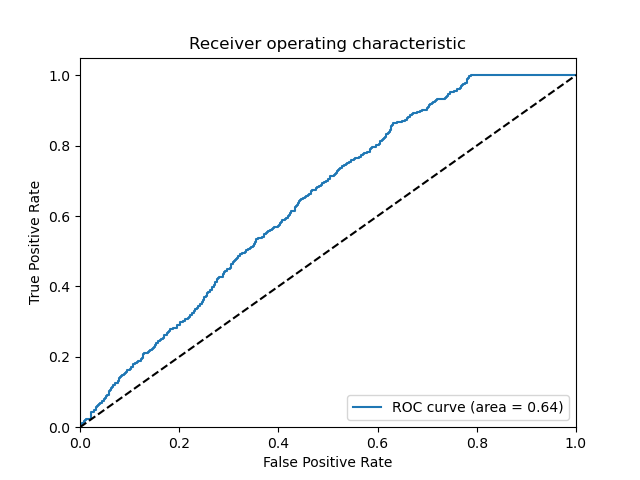
\includegraphics[width = 1.1in]{code/lr/roc_c_0.1}} &
\subfloat[$\mu$ = 0.2]{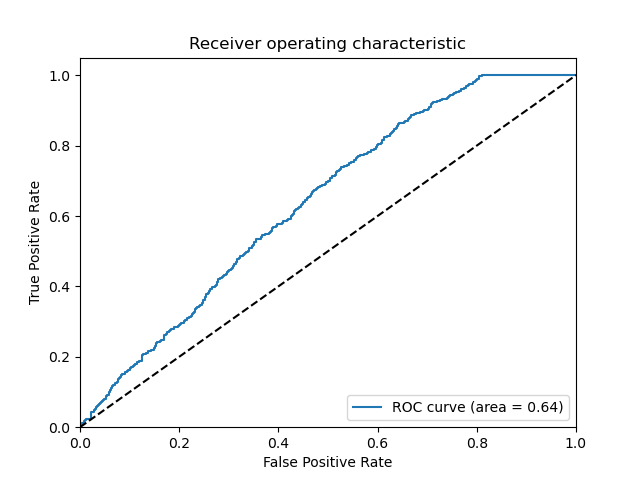
\includegraphics[width = 1.1in]{code/lr/roc_c_0.2}} &
 \subfloat[$\mu$ = 0.3]{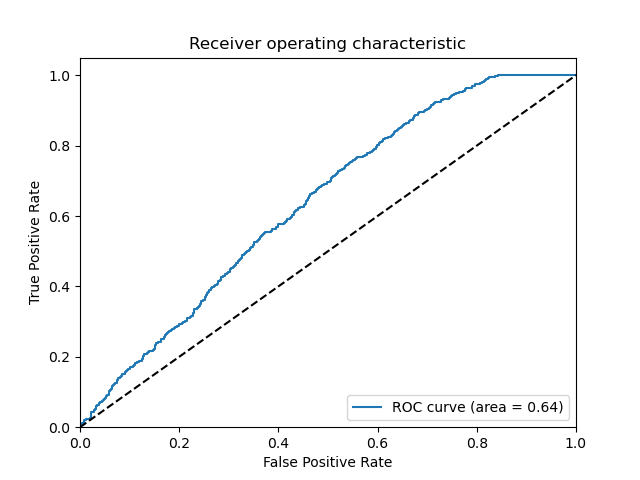
\includegraphics[width = 1.1in]{code/lr/roc_c_0.3}} &
 \subfloat[$\mu$ = 0.4]{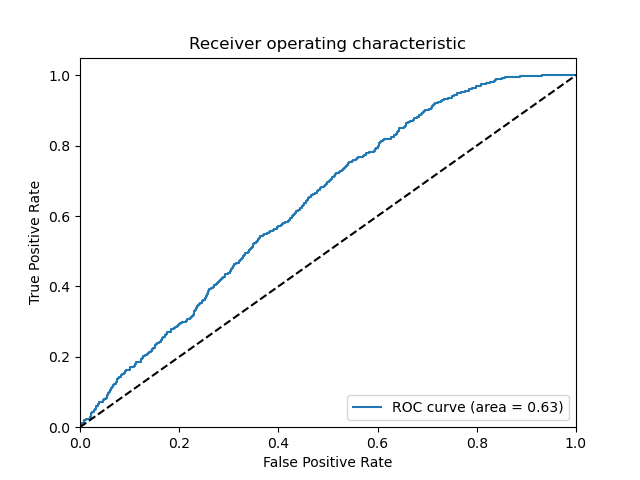
\includegraphics[width = 1.1in]{code/lr/roc_c_0.4}} &
 \subfloat[$\mu$ = 0.5]{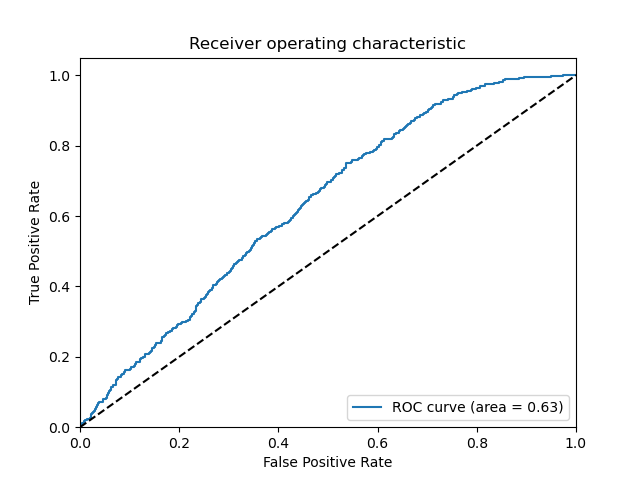
\includegraphics[width = 1.1in]{code/lr/roc_c_0.5}} \\
 \end{tabular}
\caption{ROC Curve Plots - Varying $\mu$, $\eta$=0.01}
\end{figure}

As the regularization term $\mu$ increases, the AUC decreases.  The reason for this is because $\mu$ is reducing the magnitude of the coefficients in order to prevent overfitting the model.

 \begin{figure}[h]
\begin{tabular}{ccccc}
 \subfloat[$\eta$ = 0.01]{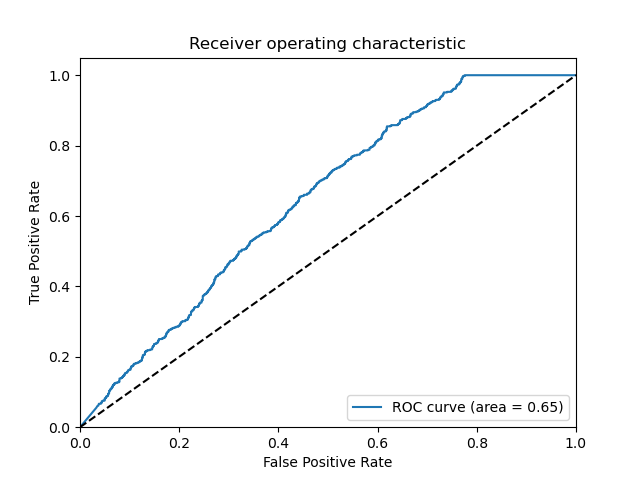
\includegraphics[width = 1.1in]{code/lr/roc_eta_0.01}} &
\subfloat[$\eta$ = 0.02]{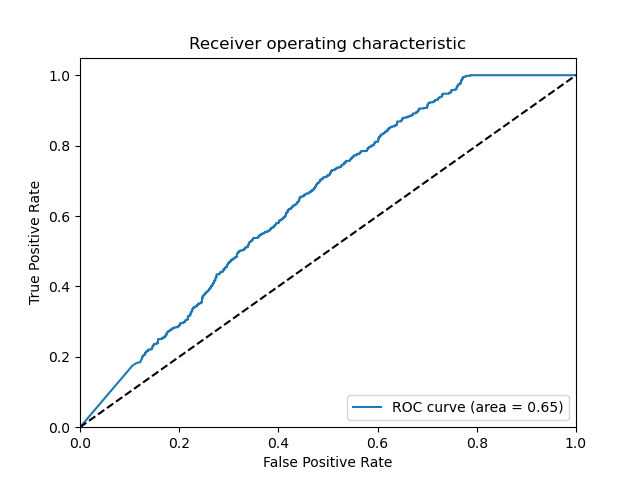
\includegraphics[width = 1.1in]{code/lr/roc_eta_0.02}} &
 \subfloat[$\eta$ = 0.03]{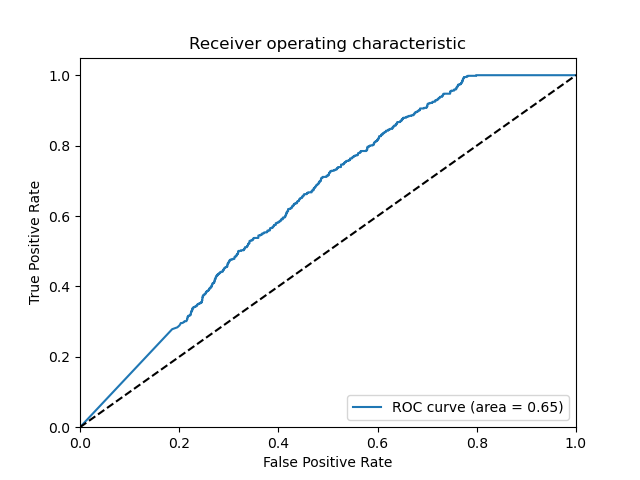
\includegraphics[width = 1.1in]{code/lr/roc_eta_0.03}} &
 \subfloat[$\eta$ = 0.04]{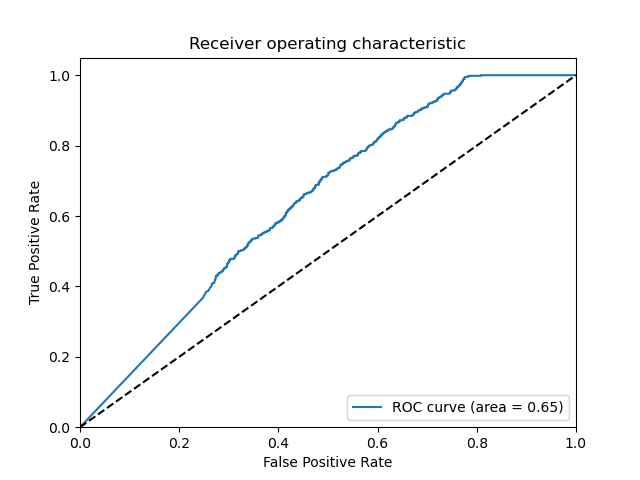
\includegraphics[width = 1.1in]{code/lr/roc_eta_0.04}} &
 \subfloat[$\eta$ = 0.05]{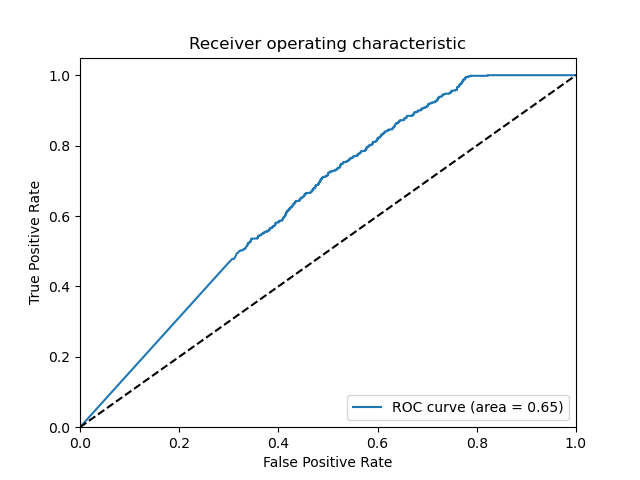
\includegraphics[width = 1.1in]{code/lr/roc_eta_0.05}} \\
\end{tabular}
\caption{ROC Curve Plots - Varying $\eta$, $\mu$=0}
\end{figure}

As $\eta$ increases, the lower left hand of the AUC curve starts off as a gradually longer straight line. Inidicating that the initial classifications are random aound a specific rate that is the slope of the curve.  As the probabilities increase, it breaks out of its random classifications and begins classify the results in a non-random manner.  This indicates that the learning rate is probably too high.

\vspace{5mm}

\iffalse
\textbf{c.} [Extra 10 points \textbf{(no partial credit!)}] Implement using the result of question \textbf{1.2.f}, and show the speed up. Test efficiency of your approach using larger data set \textit{training.data}, which has 5675 possible distinct features. Save the code in a new file lrsgd\_fast.py. We will test whether your code can finish witin reasonable amount of time and correctness of trained model. The training and testing data set can be downloaded from:

\begin{lstlisting}[frame=single,language=bash]
http://sunlab.org/download/course/hw2/training.data
http://sunlab.org/download/course/hw2/testing.data
\end{lstlisting}
\textbf{Deliverable: lr/lrsgd.py and optional lr/lrsgd\_fast.py [15 points]}
\fi

\textbf{Deliverable: lr/lrsgd.py [20 points]}

\subsection{Hadoop [15 points]}
In this problem, you are going to train multiple logistic regression classifiers using your implementation of previous problem with Hadoop in parallel. The pseudo code of Mapper and Reducer are listed as Algorithm~\ref{algo_map} and Algorithm~\ref{algo_reduce} respectively. We have already written the code for the reducer for you. Find related files in \textit{lr} folder.

\begin{algorithm}
\SetKwFunction{Random}{Random}\SetKwFunction{Emit}{Emit}
\SetKwInOut{Input}{input}\SetKwInOut{Output}{output}
\Input{Ratio of sampling $r$, number of models $M$, input pair $(k,v)$}
\Output{key-value pairs}
\BlankLine
\For{$i\leftarrow 1$ \KwTo $M$}{
$m\leftarrow$\Random\;
\If{$m < r$}{
\Emit($i,v$)
}
}
\caption{Map function}\label{algo_map}
\end{algorithm}

\begin{algorithm}
\SetKwInOut{Input}{input}\SetKwInOut{Output}{output}
\Input{$(k,v)$}
\Output{Trained model}
Fit model on $v$\;
\caption{Reduce function}\label{algo_reduce}
\end{algorithm}
You need to copy \textit{training} (the output of Pig ETL) into HDFS using command line.
\begin{lstlisting}[language=bash,frame=single]
hdfs dfs -mkdir /hw2
hdfs dfs -put pig/training /hw2  # adjust train path as needed
\end{lstlisting}
\textbf{a.} Complete the \textbf{mapper.py} according to pseudo code. [5 points]\\
You could train 5 ensembles by invoking
\begin{lstlisting}[language=bash,frame=single]
hadoop jar \
   /usr/lib/hadoop-mapreduce/hadoop-streaming.jar \
  -D mapreduce.job.reduces=5    \
  -files lr \
  -mapper "python lr/mapper.py -n 5 -r 0.4" \
  -reducer "python lr/reducer.py -f <number of features>" \
  -input /hw2/training \
  -output /hw2/models
\end{lstlisting}
Notice that you could apply other parameters to reducer. To test the performance of ensembles, copy the trained models to local via
\begin{lstlisting}[language=bash,frame=single]
hdfs dfs -get /hw2/models
\end{lstlisting}
\textbf{b.} Complete the \textbf{testensemble.py} to generate the ROC curve. [5 points]
\begin{lstlisting}[language=bash,frame=single]
cat pig/testing/* | python lr/testensemble.py -m models
\end{lstlisting}
\textbf{c.} Compare the performance with that of previous problem and briefly analyze why the difference. [5 points]

\vspace{5mm}
 \begin{figure}[h]
{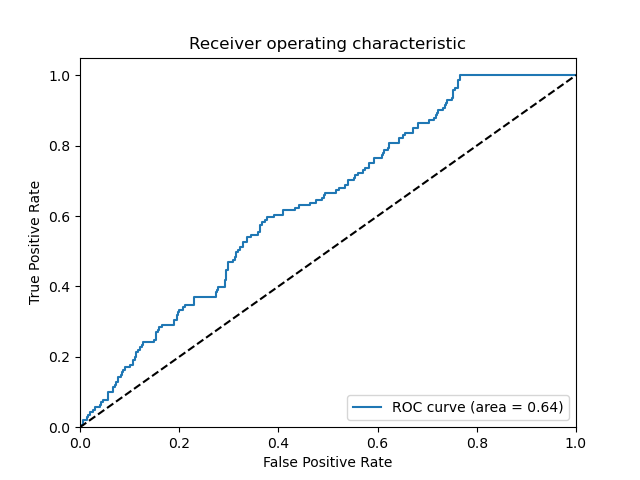
\includegraphics[width = 6in]{code/lr/testensemble_roc}}
\caption{ROC Curve Plots - Ensemble $\eta$=0.01, $\mu$=0}
\end{figure}

The ensemble method is a result of using bagging (sampling with replacement). There were 5 bags used and the average of the models predict probabilities were used create a prediction.  Since we are not using the full data set, the sampled curve tends to have meander about the true curve, resulting in a curve that is slightly different than would be attained by running the full dataset.

\iffalse
\subsection{Zeppelin [10 points]}
\href{http://zeppelin.apache.org/}{Apache Zeppelin} is an web based notebook that enables interactive data analytics (like Jupyter).
Because you can execute your code piecewise interactively, you're encouraged to use this at the initial stage your development for fast prototyping and initial data exploration. Check out the course lab \href{http://www.sunlab.org/teaching/cse6250/spring2018/lab/zeppelin-intro/}{pages} for a brief introduction on how to set it up and use it. Please fill in the TODO section of the JSON file, \texttt{zeppelin\textbackslash bdh\_hw2\_zeppelin.json}. Import this notebook file on Zeppelin first.
For easier start, we will read in the dataset we have been using in the lab, events.csv and mortality.csv, first in this part. Read carefully the provided comments in the Notebook and fill-in the TODO section:

\begin{itemize}
\item \textbf{Event count}: Number of events recorded for a given patient. Note that every line in the input file is an event. [3 points]
\item For the average, maximum and minimum event counts, show the breakdown by dead or alive. Produce a chart like below (please note that values and axis labels here are for illustrative purposes only and maybe different with the actual data): [2 points]\\
\includegraphics[width=\textwidth]{Events.png}
\item \textbf{Encounter count}: Count of unique dates on which a given patient visited the ICU. All the events: DIAG, LAB and DRUG - should be considered as ICU visiting events.[3 points]
\item For the average, maximum and minimum encounter counts, show the breakdown by dead or alive. Produce a chart like below (please note that values and axis labels here are for illustrative purposes only and maybe different with the actual data): [2 points]\\
\includegraphics[width=\textwidth]{Encounters.png}
\end{itemize}
Fill in the indicated TODOs in the notebook using ONLY Scala.\\

Please be aware that \textbf{\color{red} you are NOT allowed to change the filename and any existing function declarations.}\\

The submission bdh\_hw2\_zeppelin.json file should have all cells run and charts visible. Please don't clear the cell output before submission.

\textbf{Deliverable: \texttt{zeppelin\textbackslash bdh\_hw2\_zeppelin.json}[10 points]}
\fi

\subsection{Submission [5 points]}
The folder structure of your submission should be as below. You can display fold structure using \textit{tree} command. All other unrelated files will be discarded during testing.
Please make sure your code can compile/run normally, otherwise you will get full penalty without comments. Organize your files same as the below framework, otherwise you will get 0/5 for Submission part.
\begin{lstlisting}[language=bash,frame=single]
<your gtid>-<your gt account>-hw2
|-- code
| |-- hive
| | \-- event_statistics.hql
| |-- lr
| | |-- lrsgd.py
| | |-- mapper.py
| | \-- testensemble.py
| |-- pig
| |  |-- etl.pig
| |  \-- utils.py
\-- homework2_answer.pdf
\end{lstlisting}

Please create this folder manually, put all the files inside the folder, and create a tar archive using the following command and submit the tar file (keep in mind the folder '$<your GTid>$-$<your GT account>$-hw2' is required before creating the tar file) onto Canvas (Hadoop is not well supported on Gradescope now).
\begin{lstlisting}[language=bash,frame=single]
tar -czvf <your GTid>-<your GT account>-hw2.tar.gz \
  <your GTid>-<your GT account>-hw2
\end{lstlisting}
Example submission: 901234567-gburdell3-hw2.tar.gz
\newline

\noindent Common Errors which are not accepted:
\begin{itemize}
\item Underscore: 901234567\_gburdell3\_hw2.tar.gz   
\item Tar the files directly and rename the archive
\item Zip format is not accepted
\item Wrong submission: whoever submits your HW2 by mistake will get 0 and late policy will also apply if you resubmit it later
\end{itemize}
\end{document}
\end{document}